\begin{frame}{Միջակայքային ներկում չունեցող երկկողմանի մուլտիգրաֆներ}
\begin{theorem}[3.5.3]
Եթե $G$-ն կապակցված երկկողմանի մուլտիգրաֆ է, ընդ որում $\vert V(G)\vert\leq 4$, ապա $G\in \mathfrak{N}$: Իսկ ցանկացած $n \geq 5$ թվի համար գոյություն ունի $G$ կապակցված երկկողմանի մուլտիգրաֆ, որի համար $G\notin \mathfrak{N}$ և $|V(G)|=n$:
\end{theorem}

\begin{figure}[h]
\begin{center}
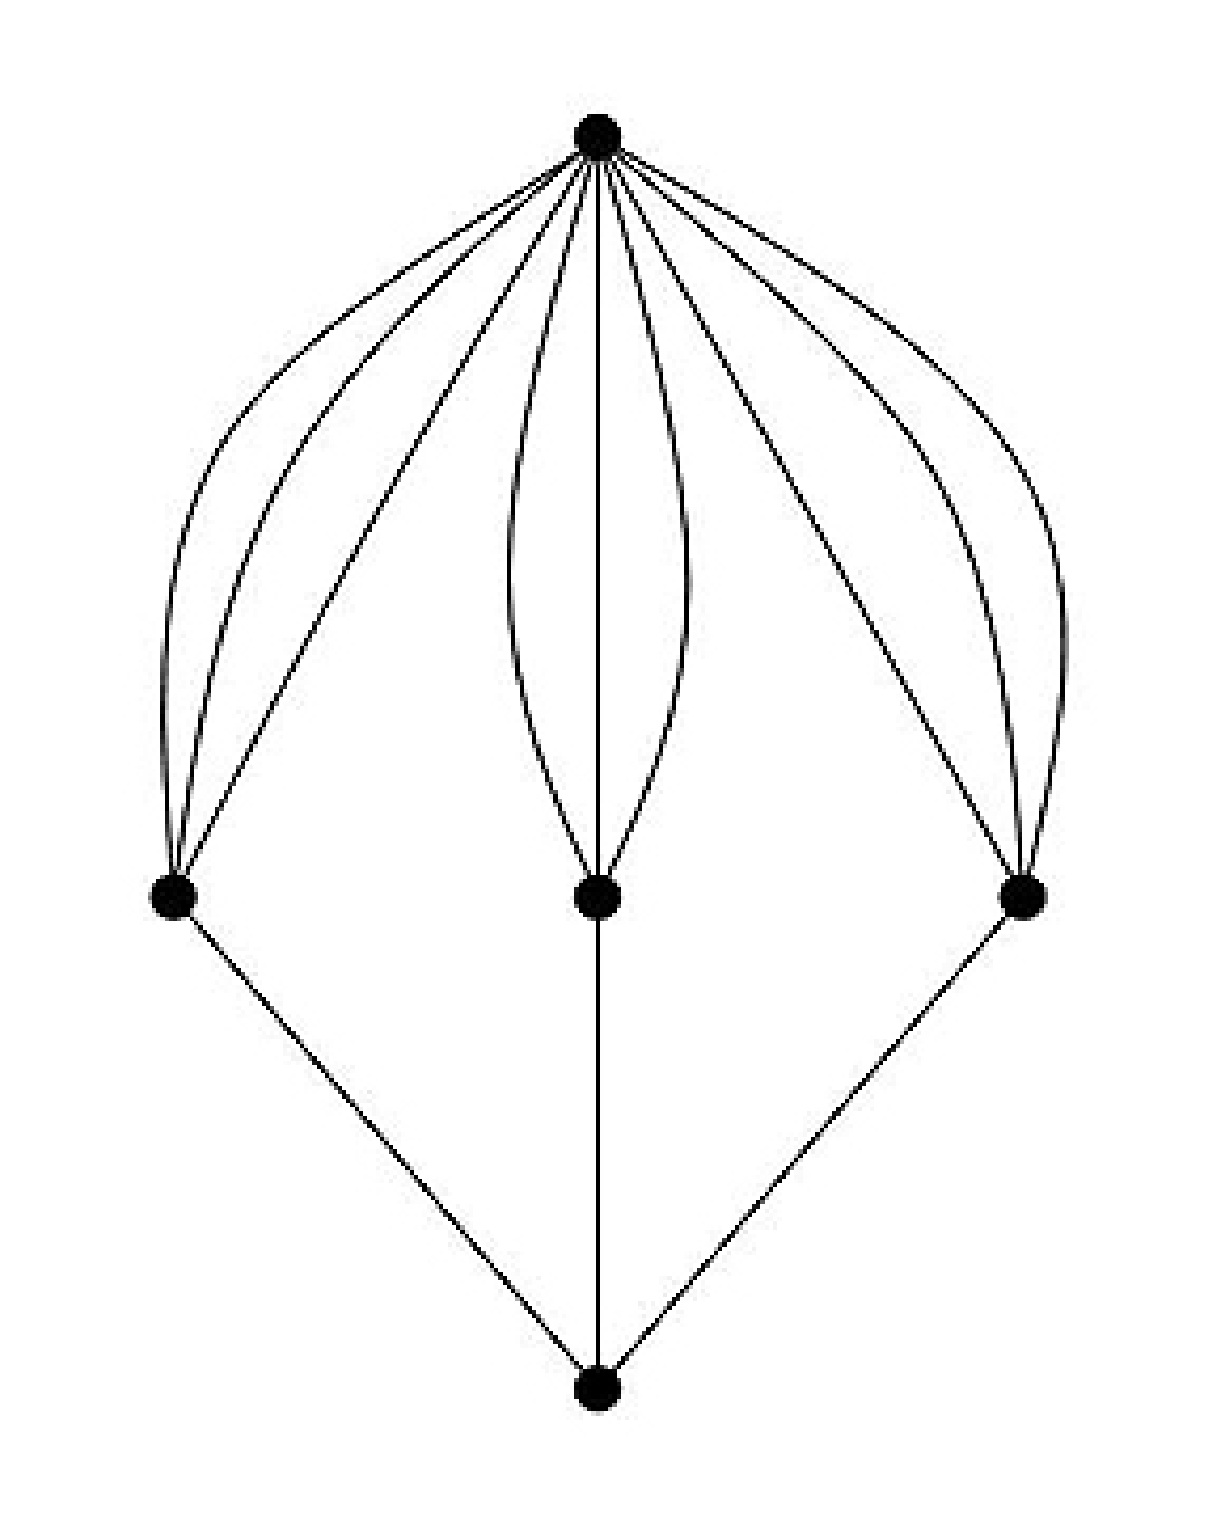
\includegraphics[width=0.25\textwidth]{figures/parachute.eps}
\end{center}
\end{figure}
\end{frame}

\begin{frame}{Միջակայքային ներկում չունեցող երկկողմանի մուլտիգրաֆներ}


\begin{figure}[h]
\begin{center}
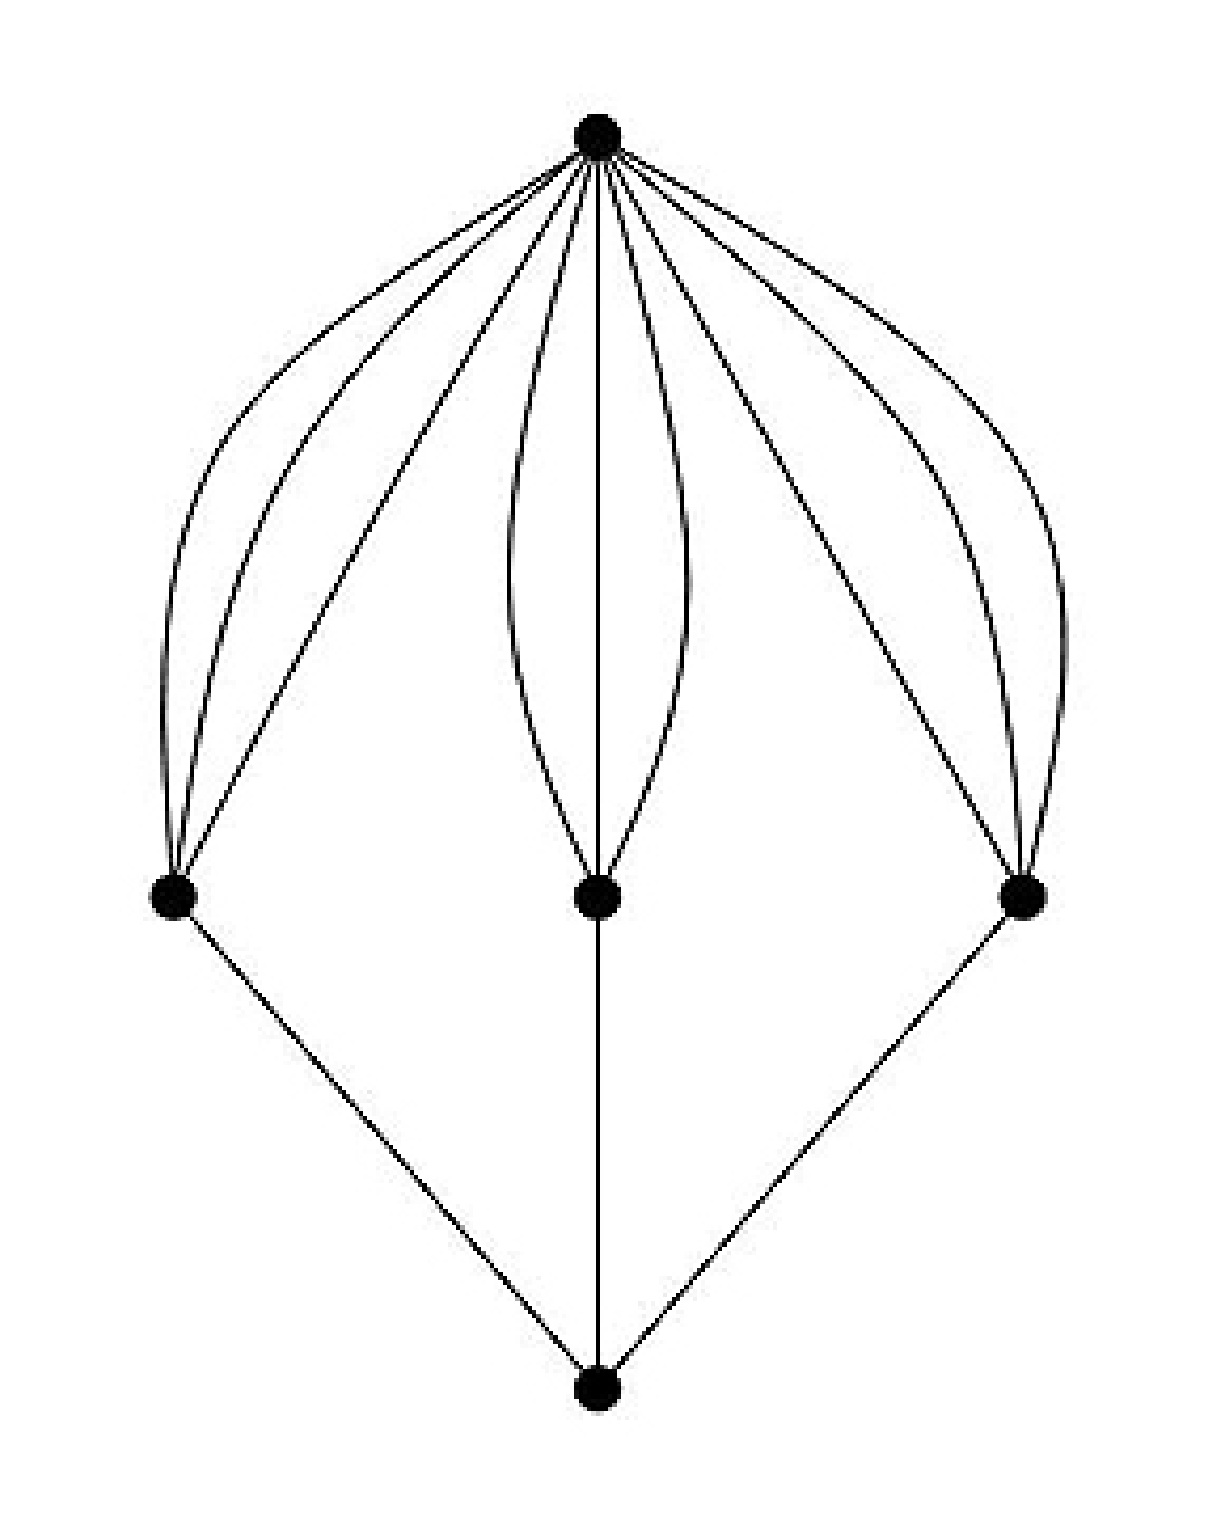
\includegraphics[width=0.25\textwidth]{figures/parachute.eps}
\end{center}
\end{figure}

\begin{theorem}[3.5.4]
Եթե $G$-ն երկկողմանի մուլտիգրաֆ է, որի համար
$\Delta(G)\leq 3$, ապա $G\in \mathfrak{N}$ և $w(G)\leq 4$: Իսկ ցանկացած $\Delta \geq 9$ թվի համար գոյություն ունի $G$ կապակցված երկկողմանի մուլտիգրաֆ, որի համար $G\notin \mathfrak{N}$ և $\Delta(G)=\Delta$:
\end{theorem}

\end{frame}